% 2008 年江苏卷第 16 题：四面体 ABCD，CB=CD，AD⊥BD，E、F 为 AB、BD 中点。
% 来源 PDF：gaokaomath-src/普通高考/2008/2008江苏.pdf
% SHA-256：b998b93963143559a1ce800a6d320de618883b0e22ee5130b7666a2374caeba0
% 原页：2008江苏.pdf 第 1 页（A3 三栏）第 2 栏，书页码 457。
% 绘制依据：按原页斜投影：B 在上、C 在左下、A 在右下、D 在内部（被遮挡）；
%   可见棱 BC、BA、CA 实线，BD、AD、CD 与 EF 虚线，E 在 AB 上、F 在 BD 上。
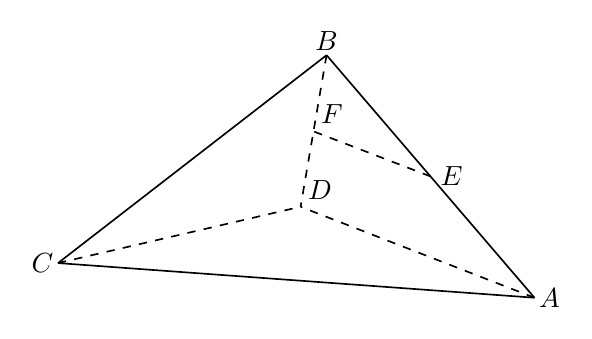
\begin{tikzpicture}[scale=1.1, semithick, every node/.style={inner sep=1.4pt}]
  \coordinate (B) at (3.6,3.3);
  \coordinate (C) at (0.5,0.9);
  \coordinate (A) at (6.0,0.5);
  \coordinate (D) at (3.3,1.55);
  \coordinate (E) at (4.8,1.9);
  \coordinate (F) at (3.45,2.42);

  \draw (B) -- (C);
  \draw (B) -- (A);
  \draw (C) -- (A);

  \draw[dashed] (B) -- (D);
  \draw[dashed] (A) -- (D);
  \draw[dashed] (C) -- (D);
  \draw[dashed] (E) -- (F);

  \node[above] at (B) {$B$};
  \node[left] at (C) {$C$};
  \node[right] at (A) {$A$};
  \node[above right=1pt] at (D) {$D$};
  \node[right=2pt] at (E) {$E$};
  \node[above right=1pt] at (F) {$F$};
\end{tikzpicture}
